\section{Introduction}

% The \textit{proceedings} are the records of a conference.\footnote{This
%   is a footnote}  ACM seeks
% to give these conference by-products a uniform, high-quality
% appearance.  To do this, ACM has some rigid requirements for the
% format of the proceedings documents: there is a specified format
% (balanced double columns), a specified set of fonts (Arial or
% Helvetica and Times Roman) in certain specified sizes, a specified
% live area, centered on the page, specified size of margins, specified
% column width and gutter size.

\begin{itemize}
\item[$\square$] A list of contribution
\item[$\square$] RQs
\item[$\square$] Settings of the study
\item[$\square$] What is the problem?
\item[$\square$] Why do you care?
\item[$\square$] Why did others fail?
\item[$\square$] What are you doing?
\item[$\square$] What did you find?
\item[$\square$] So what?
% \item[$\boxtimes$] A closed item.
\end{itemize}


Within software engineering, the term context has been used implicitly and explicitly to describe the perspective gained from all relevant information. Although we intuitively understand the notion of context, refining that into an operational framework has proved elusive. And due to this difficulty in defining context, two schools of thought have emerged -- representational context and interactional context. 
 
The representational view of context adheres to notion that context is tangible, delineable, and stable [Dourish et al. (2004), Schilit et al. (1994), Dey et al. (1999) and Pascoe (1998)]. Operationalizing this view, researchers have described context as being encoded by artifacts, tasks, and environmental factors. However, these models fail to answer the question, “what is context?” Can context be defined as the sum of all of its parts? Or is there other elements that add to context, but are not contained within it? 

The interactional view defines context as a relational property that holds between objects or activities. This view holds that activities are not disjoint from the context, but instead allow context to arise from activities [Dourish et al. (2004)]. Because of this intertwined relationship, contextual factors must be defined dynamically for each activity, and the sequence in which they occur becomes important to the definition [Viriyakattiyaporn and Murphy (2010)].

Although the interactional view of context appears to intuitively be a more accurate definition, the elements included in the definition are difficult to measure and operationalize. In this paper, we explore whether observing the interactions that occur when a programmer solves a programming task can provide insights into how context is created and evolved. 

The contributions of this paper are:
\begin{itemize}

\item We attempt to understand what artifacts and information are within the context leading to a solution. There is a pattern in which the users gain and interact with the artifacts based on the problem they are trying to solve. This gives us insights into what information from an artifact is contextualized in certain cases.

\item We attempt to understand how each information contributes to the  ideation of the solution to discover factors (other than word similarity) that affect the value associated with information. This gives us insight into how to meaning and applicability to a problem add or reduce value of information.
% Mapping goes to the next paper. For now forget about mapping.

\item We categorize the interactions as situated or planned and observe how this distinction affects the further interactions. Planned actions are often interrupted by situated ones, causing developers to pursue tasks other than they planned. In some cases this causes interruption whereas in others it aids the planned action by providing more contextualized information. 

One take-away point of the paper is what constitutes a context that guides the developer's design and implementation of a solution.

\end{itemize}



% Typically, the body of a paper is organized into a hierarchical
% structure, with numbered or unnumbered headings for sections,
% subsections, sub-subsections, and even smaller sections.  The command
% \texttt{{\char'134}section} that precedes this paragraph is part of
% such a hierarchy.\footnote{This is a footnote.} \LaTeX\ handles the
% numbering and placement of these headings for you, when you use the
% appropriate heading commands around the titles of the headings.  If
% you want a sub-subsection or smaller part to be unnumbered in your
% output, simply append an asterisk to the command name.  Examples of
% both numbered and unnumbered headings will appear throughout the
% balance of this sample document.

% Because the entire article is contained in the \textbf{document}
% environment, you can indicate the start of a new paragraph with a
% blank line in your input file; that is why this sentence forms a
% separate paragraph.

% \subsection{Type Changes and {\itshape Special} Characters}

% We have already seen several typeface changes in this sample.  You can
% indicate italicized words or phrases in your text with the command
% \texttt{{\char'134}textit}; emboldening with the command
% \texttt{{\char'134}textbf} and typewriter-style (for instance, for
% computer code) with \texttt{{\char'134}texttt}.  But remember, you do
% not have to indicate typestyle changes when such changes are part of
% the \textit{structural} elements of your article; for instance, the
% heading of this subsection will be in a sans serif\footnote{Another
%   footnote here.  Let's make this a rather long one to see how it
%   looks.} typeface, but that is handled by the document class file.
% Take care with the use of\footnote{Another footnote.}  the
% curly braces in typeface changes; they mark the beginning and end of
% the text that is to be in the different typeface.

% You can use whatever symbols, accented characters, or non-English
% characters you need anywhere in your document; you can find a complete
% list of what is available in the \textit{\LaTeX\ User's Guide}
% \cite{Lamport:LaTeX}.

% % \subsection{Math Equations}
% You may want to display math equations in three distinct styles:
% inline, numbered or non-numbered display.  Each of
% the three are discussed in the next sections.

% % \subsubsection{Inline (In-text) Equations}
% A formula that appears in the running text is called an
% inline or in-text formula.  It is produced by the
% \textbf{math} environment, which can be
% invoked with the usual \texttt{{\char'134}begin\,\ldots{\char'134}end}
% construction or with the short form \texttt{\$\,\ldots\$}. You
% can use any of the symbols and structures,
% from $\alpha$ to $\omega$, available in
% \LaTeX~\cite{Lamport:LaTeX}; this section will simply show a
% few examples of in-text equations in context. Notice how
% this equation:
% \begin{math}
%   \lim_{n\rightarrow \infty}x=0
% \end{math},
% set here in in-line math style, looks slightly different when
% set in display style.  (See next section).

% \subsubsection{Display Equations}
% A numbered display equation---one set off by vertical space from the
% text and centered horizontally---is produced by the \textbf{equation}
% environment. An unnumbered display equation is produced by the
% \textbf{displaymath} environment.

% Again, in either environment, you can use any of the symbols
% and structures available in \LaTeX\@; this section will just
% give a couple of examples of display equations in context.
% First, consider the equation, shown as an inline equation above:
% \begin{equation}
%   \lim_{n\rightarrow \infty}x=0
% \end{equation}
% Notice how it is formatted somewhat differently in
% the \textbf{displaymath}
% environment.  Now, we'll enter an unnumbered equation:
% \begin{displaymath}
%   \sum_{i=0}^{\infty} x + 1
% \end{displaymath}
% and follow it with another numbered equation:
% \begin{equation}
%   \sum_{i=0}^{\infty}x_i=\int_{0}^{\pi+2} f
% \end{equation}
% just to demonstrate \LaTeX's able handling of numbering.

% \subsection{Citations}
% Citations to articles~\cite{bowman:reasoning,
% clark:pct, braams:babel, herlihy:methodology},
% conference proceedings~\cite{clark:pct} or maybe
% books \cite{Lamport:LaTeX, salas:calculus} listed
% in the Bibliography section of your
% article will occur throughout the text of your article.
% You should use BibTeX to automatically produce this bibliography;
% you simply need to insert one of several citation commands with
% a key of the item cited in the proper location in
% the \texttt{.tex} file~\cite{Lamport:LaTeX}.
% The key is a short reference you invent to uniquely
% identify each work; in this sample document, the key is
% the first author's surname and a
% word from the title.  This identifying key is included
% with each item in the \texttt{.bib} file for your article.

% The details of the construction of the \texttt{.bib} file
% are beyond the scope of this sample document, but more
% information can be found in the \textit{Author's Guide},
% and exhaustive details in the \textit{\LaTeX\ User's
% Guide} by Lamport~\shortcite{Lamport:LaTeX}.

% This article shows only the plainest form
% of the citation command, using \texttt{{\char'134}cite}.

% Some examples.  A paginated journal article \cite{Abril07}, an enumerated
% journal article \cite{Cohen07}, a reference to an entire issue \cite{JCohen96},
% a monograph (whole book) \cite{Kosiur01}, a monograph/whole book in a series (see 2a in spec. document)
% \cite{Harel79}, a divisible-book such as an anthology or compilation \cite{Editor00}
% followed by the same example, however we only output the series if the volume number is given
% \cite{Editor00a} (so Editor00a's series should NOT be present since it has no vol. no.),
% a chapter in a divisible book \cite{Spector90}, a chapter in a divisible book
% in a series \cite{Douglass98}, a multi-volume work as book \cite{Knuth97},
% an article in a proceedings (of a conference, symposium, workshop for example)
% (paginated proceedings article) \cite{Andler79}, a proceedings article
% with all possible elements \cite{Smith10}, an example of an enumerated
% proceedings article \cite{VanGundy07},
% an informally published work \cite{Harel78}, a doctoral dissertation \cite{Clarkson85},
% a master's thesis: \cite{anisi03}, an online document / world wide web
% resource \cite{Thornburg01, Ablamowicz07, Poker06}, a video game (Case 1) \cite{Obama08} and (Case 2) \cite{Novak03}
% and \cite{Lee05} and (Case 3) a patent \cite{JoeScientist001},
% work accepted for publication \cite{rous08}, 'YYYYb'-test for prolific author
% \cite{SaeediMEJ10} and \cite{SaeediJETC10}. Other cites might contain
% 'duplicate' DOI and URLs (some SIAM articles) \cite{Kirschmer:2010:AEI:1958016.1958018}.
% Boris / Barbara Beeton: multi-volume works as books
% \cite{MR781536} and \cite{MR781537}.

% A couple of citations with DOIs: \cite{2004:ITE:1009386.1010128,
%   Kirschmer:2010:AEI:1958016.1958018}. 

% Online citations: \cite{TUGInstmem, Thornburg01, CTANacmart}.  


% \subsection{Tables}
% Because tables cannot be split across pages, the best
% placement for them is typically the top of the page
% nearest their initial cite.  To
% ensure this proper ``floating'' placement of tables, use the
% environment \textbf{table} to enclose the table's contents and
% the table caption.  The contents of the table itself must go
% in the \textbf{tabular} environment, to
% be aligned properly in rows and columns, with the desired
% horizontal and vertical rules.  Again, detailed instructions
% on \textbf{tabular} material
% are found in the \textit{\LaTeX\ User's Guide}.

% Immediately following this sentence is the point at which
% Table~\ref{tab:freq} is included in the input file; compare the
% placement of the table here with the table in the printed
% output of this document.

% \begin{table}
%   \caption{Frequency of Special Characters}
%   \label{tab:freq}
%   \begin{tabular}{ccl}
%     \toprule
%     Non-English or Math&Frequency&Comments\\
%     \midrule
%     \O & 1 in 1,000& For Swedish names\\
%     $\pi$ & 1 in 5& Common in math\\
%     \$ & 4 in 5 & Used in business\\
%     $\Psi^2_1$ & 1 in 40,000& Unexplained usage\\
%   \bottomrule
% \end{tabular}
% \end{table}

% To set a wider table, which takes up the whole width of the page's
% live area, use the environment \textbf{table*} to enclose the table's
% contents and the table caption.  As with a single-column table, this
% wide table will ``float'' to a location deemed more desirable.
% Immediately following this sentence is the point at which
% Table~\ref{tab:commands} is included in the input file; again, it is
% instructive to compare the placement of the table here with the table
% in the printed output of this document.


% \begin{table*}
%   \caption{Some Typical Commands}
%   \label{tab:commands}
%   \begin{tabular}{ccl}
%     \toprule
%     Command &A Number & Comments\\
%     \midrule
%     \texttt{{\char'134}author} & 100& Author \\
%     \texttt{{\char'134}table}& 300 & For tables\\
%     \texttt{{\char'134}table*}& 400& For wider tables\\
%     \bottomrule
%   \end{tabular}
% \end{table*}
% % end the environment with {table*}, NOTE not {table}!

% It is strongly recommended to use the package booktabs~\cite{Fear05}
% and follow its main principles of typography with respect to tables:
% \begin{enumerate}
% \item Never, ever use vertical rules.
% \item Never use double rules.
% \end{enumerate}
% It is also a good idea not to overuse horizontal rules.


% \subsection{Figures}

% Like tables, figures cannot be split across pages; the best placement
% for them is typically the top or the bottom of the page nearest their
% initial cite.  To ensure this proper ``floating'' placement of
% figures, use the environment \textbf{figure} to enclose the figure and
% its caption.

% This sample document contains examples of \texttt{.eps} files to be
% displayable with \LaTeX.  If you work with pdf\LaTeX, use files in the
% \texttt{.pdf} format.  Note that most modern \TeX\ systems will convert
% \texttt{.eps} to \texttt{.pdf} for you on the fly.  More details on
% each of these are found in the \textit{Author's Guide}.

% \begin{figure}
% 
\includegraphics{fly}
% \caption{A sample black and white graphic.}
% \end{figure}

% \begin{figure}
% 
\includegraphics[height=1in, width=1in]{fly}
% \caption{A sample black and white graphic
% that has been resized with the \texttt{includegraphics} command.}
% \end{figure}


% As was the case with tables, you may want a figure that spans two
% columns.  To do this, and still to ensure proper ``floating''
% placement of tables, use the environment \textbf{figure*} to enclose
% the figure and its caption.  And don't forget to end the environment
% with \textbf{figure*}, not \textbf{figure}!

% \begin{figure*}
% 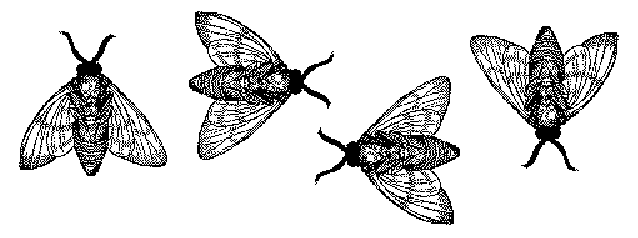
\includegraphics{flies}
% \caption{A sample black and white graphic
% that needs to span two columns of text.}
% \end{figure*}


% \begin{figure}
% 
\includegraphics[height=1in, width=1in]{rosette}
% \caption{A sample black and white graphic that has
% been resized with the \texttt{includegraphics} command.}
% \end{figure}

% \subsection{Theorem-like Constructs}

% Other common constructs that may occur in your article are the forms
% for logical constructs like theorems, axioms, corollaries and proofs.
% ACM uses two types of these constructs:  theorem-like and
% definition-like.

% Here is a theorem:
% \begin{theorem}
%   Let $f$ be continuous on $[a,b]$.  If $G$ is
%   an antiderivative for $f$ on $[a,b]$, then
%   \begin{displaymath}
%     \int^b_af(t)\,dt = G(b) - G(a).
%   \end{displaymath}
% \end{theorem}

% Here is a definition:
% \begin{definition}
%   If $z$ is irrational, then by $e^z$ we mean the
%   unique number that has
%   logarithm $z$:
%   \begin{displaymath}
%     \log e^z = z.
%   \end{displaymath}
% \end{definition}

% The pre-defined theorem-like constructs are \textbf{theorem},
% \textbf{conjecture}, \textbf{proposition}, \textbf{lemma} and
% \textbf{corollary}.  The pre-defined de\-fi\-ni\-ti\-on-like constructs are
% \textbf{example} and \textbf{definition}.  You can add your own
% constructs using the \textsl{amsthm} interface~\cite{Amsthm15}.  The
% styles used in the \verb|\theoremstyle| command are \textbf{acmplain}
% and \textbf{acmdefinition}.

% Another construct is \textbf{proof}, for example,

% \begin{proof}
%   Suppose on the contrary there exists a real number $L$ such that
%   \begin{displaymath}
%     \lim_{x\rightarrow\infty} \frac{f(x)}{g(x)} = L.
%   \end{displaymath}
%   Then
%   \begin{displaymath}
%     l=\lim_{x\rightarrow c} f(x)
%     = \lim_{x\rightarrow c}
%     \left[ g{x} \cdot \frac{f(x)}{g(x)} \right ]
%     = \lim_{x\rightarrow c} g(x) \cdot \lim_{x\rightarrow c}
%     \frac{f(x)}{g(x)} = 0\cdot L = 0,
%   \end{displaymath}
%   which contradicts our assumption that $l\neq 0$.
% \end{proof}

% \section{Conclusions}
% This paragraph will end the body of this sample document.
% Remember that you might still have Acknowledgments or
% Appendices; brief samples of these
% follow.  There is still the Bibliography to deal with; and
% we will make a disclaimer about that here: with the exception
% of the reference to the \LaTeX\ book, the citations in
% this paper are to articles which have nothing to
% do with the present subject and are used as
% examples only.
% %\end{document}  % This is where a 'short' article might terminate



% \appendix
% %Appendix A
% \section{Headings in Appendices}
% The rules about hierarchical headings discussed above for
% the body of the article are different in the appendices.
% In the \textbf{appendix} environment, the command
% \textbf{section} is used to
% indicate the start of each Appendix, with alphabetic order
% designation (i.e., the first is A, the second B, etc.) and
% a title (if you include one).  So, if you need
% hierarchical structure
% \textit{within} an Appendix, start with \textbf{subsection} as the
% highest level. Here is an outline of the body of this
% document in Appendix-appropriate form:
% \subsection{Introduction}
% \subsection{The Body of the Paper}
% \subsubsection{Type Changes and  Special Characters}
% \subsubsection{Math Equations}
% \paragraph{Inline (In-text) Equations}
% \paragraph{Display Equations}
% \subsubsection{Citations}
% \subsubsection{Tables}
% \subsubsection{Figures}
% \subsubsection{Theorem-like Constructs}
% \subsubsection*{A Caveat for the \TeX\ Expert}
% \subsection{Conclusions}
% \subsection{References}
% Generated by bibtex from your \texttt{.bib} file.  Run latex,
% then bibtex, then latex twice (to resolve references)
% to create the \texttt{.bbl} file.  Insert that \texttt{.bbl}
% file into the \texttt{.tex} source file and comment out
% the command \texttt{{\char'134}thebibliography}.
% % This next section command marks the start of
% % Appendix B, and does not continue the present hierarchy
% \section{More Help for the Hardy}

% Of course, reading the source code is always useful.  The file
% \path{acmart.pdf} contains both the user guide and the commented
% code.

% \begin{acks}
%   The authors would like to thank Dr. Yuhua Li for providing the
%   MATLAB code of the \textit{BEPS} method.

%   The authors would also like to thank the anonymous referees for
%   their valuable comments and helpful suggestions. The work is
%   supported by the \grantsponsor{GS501100001809}{National Natural
%     Science Foundation of
%     China}{http://dx.doi.org/10.13039/501100001809} under Grant
%   No.:~\grantnum{GS501100001809}{61273304}
%   and~\grantnum[http://www.nnsf.cn/youngscientists]{GS501100001809}{Young
%     Scientists' Support Program}.

% \end{acks}

\section{Motivation}

\begin{itemize}
\item[$\square$] Why is the problem a problem?
\item[$\square$] A real world consequence
\end{itemize}

\subsection{Running Example}
\begin{itemize}
\item[$\square$]A persona in the setting
\end{itemize}

\subsection{Terminology}
\begin{itemize}
\item[$\square$]Terms related to the research i.e. activities, episodes etc.
\item[$\square$]Meaning of different categories of these.
\end{itemize}

\section{Results}

\subsection{Observations}
\begin{itemize}
\item[$\square$]A persona in the setting
\end{itemize}
\subsubsection{Target Shooting}

S1 was designing and building an application by himself. Throughout the observation session, S1 catered not only to the design of his solution, but also to the architecture of the system. The session was purely exploratory, S1 had some idea of how he wanted his application to be, but no firm design or implementation. The session could not be identified as `Feature Implementation' or `Debugging', both of these activities were observed interleaved. The following observations were made from the observation session:

\begin{itemize}

\item \textbf{Activities revolved around a target:} Throughout the session, a group of S1\textquotesingle s activities revolved around a target. These groups of activities and targets are easily identifiable with an abstract knowledge of the code and description of the goal. S1 followed a pattern of identifying a target and shooting  at it until the desired behavior was reached.

\vspace{5pt}

\item \textbf{Strategies of to identify targets:} We observed two prominent strategies that S1 followed to identify his targets:
\vspace{5pt}
\begin{itemize}
\item \textbf{Targets as encountered:}  Targets were identified during runtime most often. S1 would use the application to see if it behaved as desired. Any error, fault or failure was a target. In addition to that, S1 also identified certain behavior of the application that did not match his design as a target.
\vspace{5pt}
\item \textbf{Targets defined:} There was a running set of targets that S1 had. Most of these were related to all the features he wanted to implement, or changes he wanted to make in to future. Once all targets from the runtime was eliminated, S1 would fall back to the running set of defined targets. The number of targets in this set would increase or decrease with the activities. New targets are added to the list while working on other targets. But targets are rarely eliminated unless S1 exclusively worked on it.
\vspace{5pt}
\item \textbf{Sequence of targets:} There were instances during the session where a sequence of segments of activities were used to shoot targets that was identified during the immediately 2 or 3 preceding segments. These were instances where a bug covered the exposure of another bug, or when events that take place earlier another are buggy masking the bug in the succeeding event's behavior. In one instance, S1 performed a shotgun surgery leading to targets emerging one after the other.
\end{itemize}
\vspace{5pt}

\item \textbf{Target stages:} S1\textquotesingle s sequence of activities map to the various stages of evolution of his targets. Activities can be grouped according to what was happening to one or more targets. S1's observation session revealed four distinguishable stages through which the targets are identified and eliminated:

\begin{itemize}
\item \textbf{Explore:} An exploration stage starts with the target set $T = \emptyset$. This is where S1 recalled his goals from another session and from exploring the application's behavior. After this stage S1 has at least one target in the set  $T=\{t_i \mid i={1,\dots,n}\}$. 
\vspace{5pt}
\item \textbf{Identify:} When there were more that one targets in $T$, i.e. $ n(T) > 1 $, immediately after exploration S1 focused on identifying a working target $t_w, where, 1 \leq w \leq n $. S1\textquotesingle s activities during this time was mostly inspecting self code and examining existing code with long periods of scrolling and inactivity inside the IDE. The selection of $t_w$ from $T$ is based on different characteristics of the targets like ease of solving, dependency on other targets, eliminating $t_w$ eliminates other targets from the set, relevance of the target to the goal and priority of the target. At one point, S1 had 2 possible targets tied to the same goal. S1 bounced back and forth between the two targets and finally chose $t_2$ because \textit{"$t_2$ was simpler whereas $t_1$ was a behavior happening across time"}. Another time, S1 chose $t_m$ over $t_p$ even though $t_m$ was a subproblem, because \textit{"$t_m$ was a quick fix, and [S1] wanted to try it out to see what happens before moving on to $t_p$"}. Such a choice is \textbf{non-intuitive} and defies \textbf{IFT} concepts of information value.
\vspace{5pt}
\item \textbf{Edit:} When S1 found a working target $t_w$, he would edit the relevant part of the artifact. If $t_w$ was a certain cue like error declaration found during \textit{Identification} stage, S1 moved to the part of the code which contained the relevant method or line to edit. If it was an anomalous behavior that didn't match his vision, S1 moved to examine the existing code to find an entry point to the relevant part of the artifact. Once the relevant part is found, S1 edits it, or shoots the target. There were cases where S1 shot at multiple targets at once and other cases where S1 shot at a \textit{super-target}, i.e. a target having more that one sub-targets.
\vspace{5pt}
\item \textbf{Assess:} Immediately after every edit activity, S1 performed an impact assessment of the shot taken. S1 always performed \textit{Assessment} by launching his application and checking for the behavior. During this stage targets maybe eliminated i.e. reduction of target set $T=\{t_i \mid i={1,\dots,m}\}, where, m<n $. But during many cases, the shot taken at the working target $t_w$ failed to produce desired effect. In such cases where S1 aimed incorrectly, he either immediately returned to \textit{Edit} stage to shoot again or spent time in the application window marked by long periods of inactivity. These inactive periods were maybe used to reflect on why he missed the target. When the target was missed, in most cases the target set remain unchanged. However, there were cases when new targets were added even after a missed shot because it revealed new anomalous behavior causing an increase in the number of running targets in the set $T=\{t_i \mid i={1,\dots,k}\} , where, k>n $. In cases where S1 successfully eliminated a target, he either returned to identify the next working target $t_w$ from the running set of targets $T$, or it lead to a \textbf{sequential target}. S1 says such sequential targets are exposed after a target is eliminated because of \textit{"overlying bugs on top of other bugs"}. These sequential targets get added to $T$, and in most cases are relevant to the previous working target causing S1 to choose it as $t_w$. In one case, S1 decided to choose a target from the running set $T$ that wasn't a sequential target as $t_w$. S1 explained that the application behavior even with the sequential target was \textit{"good enough for the time being"} and prior running targets were more important. 
\vspace{5pt}
\end{itemize}

\item \textbf{Activities may reveal targets and target-stages:} The target stages can be clearly identified with the sequence of activities performed. E.g. Examining code [AU3] is tied to the Exploration and Identification stages, however if examining code [AU3] was followed by assessment of changes [AI5], S1 was performing Identification of working target. Similarly editing code [AI1] is mostly tied to the the target phase Edit. Yet there were instances when S1 made edits to the code [AI1] e.g. print statements to print the number of objects, following which S1 took the necessary steps on the application to see the output of the print statements. Thus, in this case, edit [AI1] followed by assessment of changes [AI5] is tied to the Identification stage of the target. \newline
It is harder to define the targets from the activities. To define the targets it is necessary to observe the artifacts being used in the activities, and often observing 2 or 3 such segments are necessary for identifying the targets. 
\end{itemize}

\subsubsection{Context in shooting} S1 maintained a context 
\subsection{Hypotheses}

\section{Implications and Future Work}

\section{Discussion and Limitations}

\section{Related Work}
\subsection{What programmers do when coding}
Kim et al. studies how Software engineers inspect program differences when reviewing other's code changes, when writing check-in comments, or when determining why a program behaves differently from expected behavior after modification ~\cite{Kim:2009}.
Prior research has identified many hard-to-answer questions developers ask as part of their development activities ~\cite{LaToza:2010, Fritz:2010, Ko:2007}. 
LaToza et al. studies what questions about code developers perceive hard to answer ~\cite{LaToza:2010}. They report that questions about the rationale~\cite{LaToza:2006} and intent of a code --- what does this code do, what is it intended to do, and why was it done this way? --- were considered the hardest to answer. 
\begin{itemize}
\item Developers look for which functionality they can reuse and how to reuse it. (T\textbf{his can be translated to developers build not only the context of reusable functions, but also the context of the act of reusing in itself}) ~\cite{Ko:2007}.

\item \textit{``Developers ask design questions about code's rationale and implications of a change"} ( \textbf{this directly translates to how developers build the contextual information which lead to the creation of the code and the contextual map of data flow})~\cite{Ko:2007}.

\item \textit{``Developers begin coding tasks by finding focus points corresponding to domain concepts or application functionality and work outward following relationships between methods and classes." }(\textbf{This maps to the information which triggers the context building or the aspects that define context of a code})~\cite{Sillito:2008}.

\item `\textit{`Developers ask higher-level questions about relationships between multiple methods and classes, including questions about control and data flow."} (\textbf{how they combine context})~\cite{Sillito:2008}.

\end{itemize}

Ko et. al. also investigated the information needs among developers by shadowing them at work~\cite{Ko:2007}. They found \textit{``The most frequently sought information included awareness about artifacts and coworkers. The most often deferred searches included knowledge about design and program behavior, such as why code was written a particular way, what a program was supposed to do, and the cause of a program state."} They also found that the most frequently sought info is perceived to be more important, whereas the more deferred info is perceived to be more unavailable.
When developers asked questions about what code elements to use to implement a behavior(c1), they were mostly searching for existing reusable code. Immediately after what, they asked how they could implement the behavior. Most cases the behavior was undocumented, and developers resorted to inferring the behavior themselves. 
When trying to understand the behavior, developers hypothesized about the cause. \textit{``Developers acquired their hypotheses (u1) by using their intuition {ALM}, asking coworkers for opinions {AFM}, looking execution logs {F}, scouring bug reports for hints {ER}, and using the debugger {GTU}.}" Ko et al. notes that \textit{``The accuracy of developers' hypotheses was only obvious in hindsight"}. But this hypothesis based development was risky and costly, since often hypotheses were false. \textit{``Instead, developers frequently assessed the value in continuing their investigation, stopping when necessary"}. Ko et al. also notes that not only did developer need to know what a program was supposed to do, but the historical reason for the current implementation was important too. They also had problems articulating the complex runtime scenarios into words or representations. Ko also pointed out that developers feel that commenting the why and not the what was something that developers realize, but don't engage in because it becomes outdated fairly quickly and is hard to maintain. Ko also says, questions about the behavior of a program is difficult because of the number of possible explanations of a certain behavior.
Ko et al. also points out that software, inherently, is more complex and it is hard to capture and document design. \textit{``code did not look like design; intent could rarely be inferred from code; programming languages only allowed a single, structural perspective on code, yet there were many other perspectives on which developers reasoned about code."} This distribution of knowledge in various people resulted in inconsistent vision of the software.

Sillito et. al.  studied programmers performing software evolution tasks and found 44 questions asked during that ~\cite{Sillito:2006}. They also discuss how the participants answer the question including how developers use tools and how they frame results from these tools. They found 4 categories : \textit{``Questions in the first category are about discovering an initial entity in the graph. Questions in the second category are about a given entity and other entities directly related to it. Questions in the third category are about understanding a number of entities and relationships together. Questions in the final category are over such connected groups; how they relate to each other or to the rest of the system"}. They rationalize their categorizing strategy by pointing out that it demonstrates the amount of info needed, captures intuition of levels of questions and show relationships between questions. Sillito et. al. found that participants often jumped around questions, leaving some of them unanswered. They struggled to find what information was relevant. Sometimes participants asked a series(linear) of question from each new entity discovered, other times they would focus on one entity and branch(star) their questions. They would also compare information from tools side by side, ask questions about impact of changes.
Sillito et al points out that devs. asked lower level question to answer higher level ones. \textit{``This question was not directly sup- ported by any of the tools available; instead the participants asked several other questions around finding candidate classes and building on those results".} \textit{``At times the lower-level questions were asked first"}. Some of these lower level question were answered by tools but often there was mismatch. \textit{``the results produced by tools were often noisy when considered in the context of the questions being asked by the participant"}. Participants wanted higher level overview by combining results from various tools. A large number of results often did not answer the original question posed. These lead participants to rethink what lower level question they should ask and often this process was long. Finally, asking and answering questions were, obviously, interleaved. \textit{``Determining relevance required additional exploration on the part of the participant. This imperfect mapping between questions and tools together with the use of multiple tools required participants to mentally piece together pieces of information from multiple (often noisy) result sets." }
In consistence with Ko et. al.'s findings Sillito et al found that the questions were very similar except for the amount of information needed to answer them ~\cite{Ko:2007,Fritz:2010,Sillito:2006}. Sillito et al also agreed with Ko et al.’s finding that participants hypothesize when determining what lower level question to ask 
Sillito’s findings regarding the 4 categories and visualizing information as sub-graph calls can be used to support context combination. If, instead of the nodes in the graphs being a question, the nodes are contexts that participants acquire, then a graph which is activated can refer to how people build a larger (or the next larger context).  

Sillito et al later extended their work to find out how much tool support is available for each of the 44 questions that developers ask ~\cite{Sillito:2008}. He found the first two categories (finding a focus point, and expanding a focus point) are well supported. The questions in the category of understanding a subgraph and groups of subgraph are only partially supported. `\textit{`We found that, often, to answer these lower level questions, possibly less refined versions of these questions (i.e., ones with better tools support) must be asked, resulting in noisier result sets and the need to mentally put together answers." ``Programmers are often limited in how precise or refined their questions can be." ``Some tools that we have shown to partially help answer higher level questions, such as impact analysis tools, simply produce a list of candidate entities to consider; investigating those can be nontrivial and generally requires using other tools." ``Programmers map their questions to multiple tools that they believe will produce information to help answer their question." ``In cases like these, the burden is on the programmer to assemble the information needed to answer their intended question, which can be difficult." }They also find cases where challenges \textit{``stemmed from various forms of indirection or the volume of information presented by the various tools."}
Begel and Zimmermann performed a large survey on Microsoft developers finding 145 questions that developers want data scientists to answer ~\cite{Begel:2014}. They found 12 concise categories for these questions. For a second survey, they asked developers to mark the 145 questions as Essential, Worthwhile, Unimportant or Unwise. Some of the highest `Essential' rank questions are\textit{ ``How do users typically use my application?"}, \textit{``What parts of a software product are most used and/or loved by customers?", ``How effective are the quality gates we run at check in?"}, \textit{``How can we improve collaboration and sharing between teams?"}. Some highest `Unwise' questions were – \textit{``Which individual measures correlate with employee productivity (e.g., employee age, tenure, engineering skills, education, promotion velocity, IQ)?"}, \textit{``Which coding measures correlate with employee productivity (e.g., lines of code, time it takes to build the software, a particular tool set, pair programming, number of hours of coding per day, language)?"}.  They found that developers are interested in questions of their domain (testers, devs etc.). Instead of managers, individual contributors wanted to measure an employee's productivity. Experienced people in general are less interested in data scientists looking at their code, because they have acquired large knowledge sharing networks through the years. Experienced managers care less about investigating impact of old code.

Fritz and Murphy proposed an information fragments model to answer questions that developers ask ~\cite{Fritz:2010}. They take a classic graph-theory approach to providing useful information that a developer seeks by defining each info. fragments as a vertex, edges between those vertices, and unique identifier for each of those vertices. A mapping function for each vertex relates the vertices to information fragments. The developer looking for a particular information can perform various composition operations to reach to a certain combined info fragment. 

While doing so, Fritz and Murphy points out that 
\begin{itemize}
\item often developers look for more than one kind of information at the same time.
\item most of the questions, although sound similar, require different pieces of info.
\item some questions require the same info, but ``there can be substantial variation in how a developer interprets a question".
\item Developers often want different presentations of the same info: each developer and a listing of their work Vs. each work and the developers involved with it.
\item ``Similar questions often just differ in small details of the information of relevance. However, this difference influences the size of the result and the ease of interpreting it."
\item One can only follow one branch of thought at a time. It is hard for developers to follow a flow chart style pattern of possible information sources.
\item ``By composing fragments, one can create the context that allows him/her to answer the question at hand."

\end{itemize}

They also interviewed developers to gather 78 questions. ``These questions span eight domains of information: source code (SC), change sets (CHS), teams (T), work items (WI), web sites and wiki pages (WW), comments on work items3 (CO), exception stack traces (ST) and test cases (TC)."  They found that ``participants reordered the information shown in the composition view more often (277 times) than the participants restarted the composition (213 times)." Note that composition operation is choosing which different info domains one wants to answer a question.

Erdos and Sneed ~\cite{Erdos:1998} suggest that only seven questions need to be answered for a programmer to maintain a program that is only partially understood:
\begin{enumerate}
\item where is a particular subroutine/procedure invoked? 
	\begin{enumerate}
	\item comes up with the ``task of correcting or adapting a particular subroutine or procedure. One must first know in what context that procedure is used, i.e. where is the procedure invoked"
	\item They suggest a fan.in diagram to that one particular procedure is required. 
    \end{enumerate}
\item	what are the arguments and results of a given function? 
	\begin{enumerate}
	\item ``maintenance programmer must change or enhance invokes a particular procedure, … what parameters are passed to that procedure and how are they processed." 
	\item ``some kind of representation of that procedure" e.g. A low level data flow diagram.
    \end{enumerate}
\item how does control-flow reach a particular location? 
	\begin{enumerate}
	\item come up when correcting errors, one ``must trace the control flow back from a given point of interest to the start of a procedure".
	\item to answer this one needs ``decision tree in which the potential points of interest are the edges and the decisions are the nodes."
    \end{enumerate}
\item where is a particular variable set, used or queried? 
	\begin{enumerate}
	\item Comes up with an attempt to alter a variable type or length. 
	\item The answer is ``a cross reference list in which all commands in all procedures which reference the target variable are listed out."
    \end{enumerate}
\item where is a particular variable declared? 
	\begin{enumerate}
	\item Accompanies location of data object.
	\item The answer is ``a data to object reference list which tells where and how the data variable is declared."
    \end{enumerate}
\item where is a particular data object accessed?
	\begin{enumerate}
	\item This ``comes up when an external data object such as a record, segment or table is altered."
	\item This needs a cross reference list.
    \end{enumerate}
\item what are the inputs and outputs of a module? 
	\begin{enumerate}
	\item All types of maintenance.
	\item Needs a high level data flow diagram.
    \end{enumerate}
\end{enumerate}

Johnson and Erdem classify these questions as goal-oriented (requested help to achieve task-specific goals), symptom-oriented (why something is going wrong) and system-oriented (requested information for identifying system objects or functions). In their model, a question is represented based on its topic (the referenced entity), question type (verification, identification, procedural, motivation, time or location) and the relation type (what sort of information is being sought) ~\cite{Johnson:1995}.

Herbsleb and Kuwana report on the types of questions asked by their participants as well as how frequently each of those questions were asked ~\cite{Herbsleb:1993}.

Breu et al looked at bug repositories to identify information needs when dealing with bugs ~\cite{Breu:2010}. They found that questions people ask when dealing with bugs belong to 8 categories: \textbf{Missing Information}(3) (``… information such as steps to reproduce, build numbers, OS, test cases, examples, program output, and screenshots"), \textbf{Clarification} (``Often developers are even clueless what problem is reported in a bug", ``want to know if they have been helpful or whether additional information is needed"), \textbf{Triaging} ( bugs are submitted to wrong component/project, two bugs reported in one, duplicate reports and who should fix), \textbf{Debugging(2)} (``developers ask questions about behavior and state of a program, and about code pieces."), \textbf{Correction }(1) (``once developers found the cause of a bug, they discuss solutions and alternatives before they fix the bug", ``questions in understanding fixes relate to an implemented solution, often a patch"), \textbf{Status Enquiry} (``progress in general or whether a fix will make a certain version or build of the program."), \textbf{Resolution} (whether bug is resolved), and \textbf{Process} (“administrative tasks, best practices, and procedures”).Breu et al. reported that the information needs of developers change as time progresses. Developers expect that users who report the bug will stick along and participate in the discussion as developers addressed questions to users throughout the bug’s life. \textit{``Most questions were aimed at understanding the issue sufficiently"}.

Roehm et al ~\cite{Roehm:2012} studied how people comprehend program. He found
\begin{itemize}
\item \textit{``Developers usually follow a recurring, structured comprehension strategy that varies with the type of task, developer personality, the amount of previous knowledge about the application and the type of application.''}
\item \textit{``Developers try to avoid comprehension by cloning pieces of code if they cannot comprehend all possible consequences of changes.''}
\item \textit{``Developers comprehend software by asking and answering questions and establishing and testing hypotheses about application behavior.''}
\item \textit{``Some developers use temporal notes as comprehension support. This externalized knowledge is only used personally. It is neither archived nor reused.''}
\end{itemize}
He also found most people source code as the source of information. Then they prefer communication over documentation. Standard naming conventions can be helpful but if too complicated, does harm. `\textit{`Knowledge about rationale of the implementer and intended ways of using a piece of code help to comprehend code but this information is rarely documented.''} They also found that in most cases programmers use IDE in parallel to specialized tool even though both give similar info, and compilers are often used to get structural information.

\subsection{Studying Programmer Behavior}
Meyer et al. ~\cite{Meyer:2017} studied programmers in their workspace and reports multiple times that a developer's work is highly fragmented and this causes a disruption flow. This break in flow causes them to lose productivity and can be interpreted by assuming that the developer had to put himself into his unfinished context or has to recreate context again. They report that developers spend most time looking for information and reading documentation and source code. Minelli et al. ~\cite{Minelli:2015} report that developers are inactive from IDE to perform program comprehension. Meyer et al. draws from their observation that ``This notion of taking a few minutes to understand, think about or read the current artifact, such as code, a website or document, is likely another reason for these short inactivities.'' They also report that developers use a large number of different apps (331 to be exact). 
``A developer's typical work day is mostly spent on coding ($21.0\%$), emails ($14.5\%$), and work-related web browsing ($11.4\%$).''  They also report that debugging, code review and version control only accounts for $2.4\%$. developers read/edit/navigate code for $21\%$, read edit documents $6.6\%$ and browse internet related to code/work/task for $11.4\%$. They further report that developers have varied notion of task definition and granularity. When switching context, developers go from code $\rightarrow$ work related browsing ($22.1\%$), code $\rightarrow$ read/write docs ($14.3\%$) and code $\rightarrow$ planning ($14.2\%$). They say this is due to the need for additional requirement needed to complete the task.

Brandt et. al. ~\cite{Brandt:2009} looked into how novice (through lab studies) and professional programmers (by analyzing month-log web query data) use web and online resources when they are programming. They reinstate that a lot of research has gone into recognizing the barriers but they ``provide insight into the problems that programmers face, there is little discussion of how programmers currently overcome these barriers.'' They point out that although many papers have tried to use data mining techniques to recommend/synthesize code snippets by leveraging context, but the ``limitation of this approach is that the generated code lacks the comments, context, and explanatory prose found in tutorials''.Brandt et. al. report that web search during programming (19\% of the time) has three intentions --- for (1) learning by doing, for (2) clarification of existing knowledge and for (3) reminding themselves of a concept they knew well. When learning by doing, the web searches are longer in time, the queries are in natural language. The search queries are refined often, even before the results are clicked. The authors state that participants often open a number of relevant websites in new tabs before refining queries. They follow IFT principles to finally choose from them. Copy and paste was used a lot from these websites. When using the web for clarification of existing knowledge, the authors state that the participants ``needed a piece of clarifying information to help map their schema to the particular situation''. This is more similar to context. The queries contained more programming language terms, copied from the resulting websites and trusted the results. This kind of web use was also frequent in cases where errors were difficult to understand. Participants also used web as a reminder for low-level syntactic details. These took the shortest time, and participants sometimes only saw the search result snippet without viewing an actual result. Alternatively, participants also kept certain pages (official documentation) open at all times, and use syntax from the webpage which are regularly used so that they don't have to memorize it. The queries were mostly code-only, and had the fewest refinements. (Not all open webpages are in context, but the mapping to the webpage is in context) 

\subsection{Concepts used to Assist Exploratory Programming}
Kim et. al. built Logical Structural Diff (LSdiff), a tool that infers systematic structural differences as logic rules. LSdiff complements existing differencing tools by grouping code changes that form systematic change patterns regardless of their distribution throughout the code, and its ability to discover anomalies shows promise in detecting inconsistent changes ~\cite{Kim:2009}. Dagenais and Robillard's SemDiff ~\cite{Dagenais:2008} monitors adaptive changes within a framework to recommend similar changes to its clients. SemDiff and LSdiff are similar in that both identify additions and deletions of methods and method-calls. Dagenais et al. automatically infer structural patterns among the participants of the same concern and represent such concerns using a rule syntax for tracing concerns over program versions.

Several approaches use change history to identify code elements that tend to change together~\cite{Gall:1998, Ying:2004, Zimmermann:2004}. One way is to help developers understand the code evolution by recording and replaying fine-grained changes in the integrated development environments (IDEs) ~\cite{Maruyama:2012, Hattori:2011, Hattori:2010}. One experiment showed that developers can answer software evolution questions more quickly and correctly when provided with a replay tool. The second way is to analyze the history data for research purposes. This approach has also been successfully used to identify programmers' common coding practices such as backtracking ~\cite{Yoon:2012} and refactoring ~\cite{Vakilian:2012}. 

Yoon et al. presented two visualizations of fine-grained code change history -- a timeline visualization, and a code his- tory diff view. The timeline and filtering options allow developers to navigate through the history. The code history diff view shows the history of any particular code fragment, allowing developers to move through the history simply by dragging the marker back and forth through the timeline to instantly see the code that was in the snippet at any point in the past ~\cite{Yoon:2013}

Approaches such as JQuery ~\cite{Janzen:2003} or CodeQuest ~\cite{Hajiyev:2006} automatically evaluate logic queries specified by programmers to assist program investigation. Mens et al.'s intentional view ~\cite{Mens:2002} allows programmers to specify concerns or design patterns using logic rules. Eichberg et al. ~\cite{Eichberg:2008} use Datalog rules to continuously enforce constraints on structural dependencies as software evolves. 

\section{Conclusion}

\section{Acknowledgements}

\section{Appendix}

\section{FAQs}